\section{Application à la fonction Level Set}


\label{sec:application}

\indent Le modèle décrit dans la section précédente a été utilisé initialement pour adapter le maillage par rapport à une fonction Level Set (LS). Cette fonction définit une distance signée entre chaque point du maillage et la surface qu'on représente: si le point \(\vecx\) est à l'extérieur de la surface, \(LS(\vecx) > 0\); s'il est à l'intérieur, \(LS(\vecx) < 0\); et si il est sur l'interface, \(LS(\vecx) = 0\).  On cherche alors à bouger les points pour avoir une meilleure représentation de la ligne de niveau 0 de la fonction Level Set, \emph{i.e.}, de la surface de l'objet \cite{ducrot}. Pour illustrer notre objectif, on présente dans la figure \ref{fig:exLS} un exemple d'adaptation à une fonction Level Set :

\indent

\begingroup
	\begin{minipage}[t]{.5\linewidth}
		\centering
		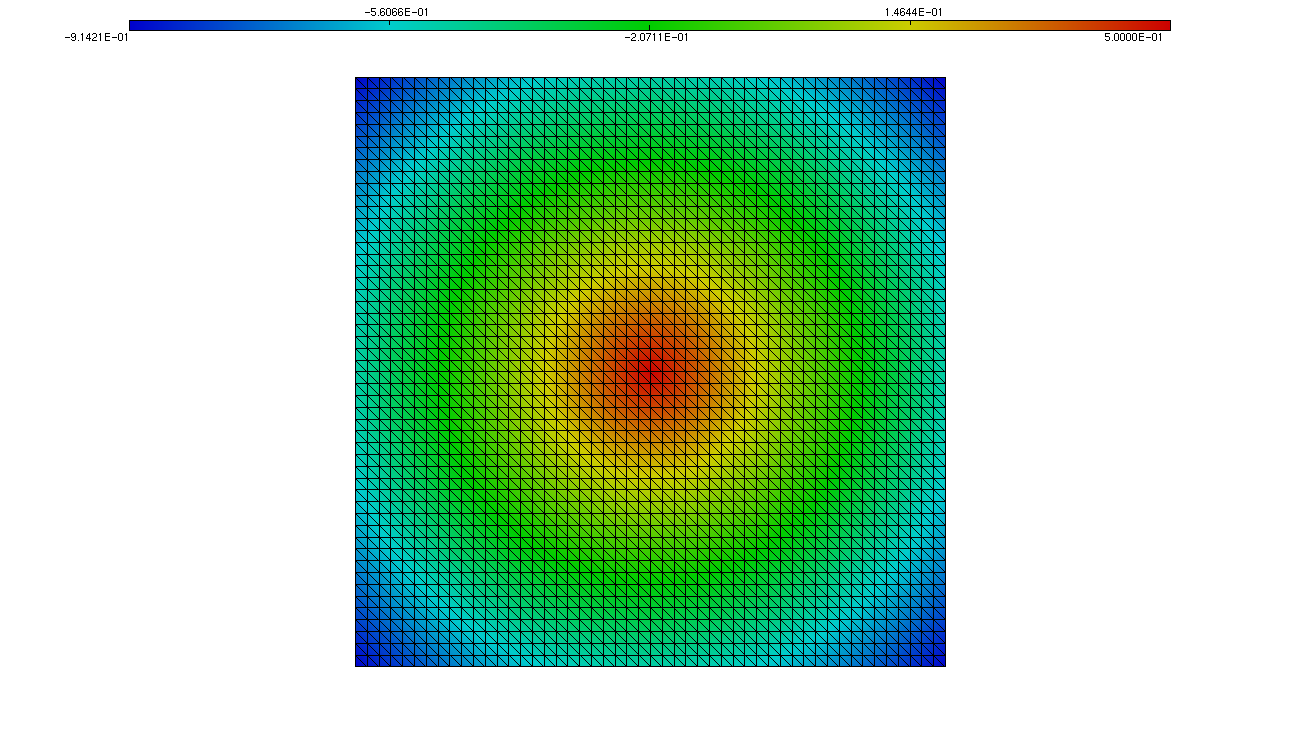
\includegraphics[clip=true, trim = 10cm 0 10cm 0, scale=.25]{Bordeaux/figures/LSinit.png}
		\captionof{subfigure}{Fonction Level Set représentée sur le maillage initial}
	\end{minipage}
	\hfill
	\begin{minipage}[t]{.5\linewidth}
		\centering
		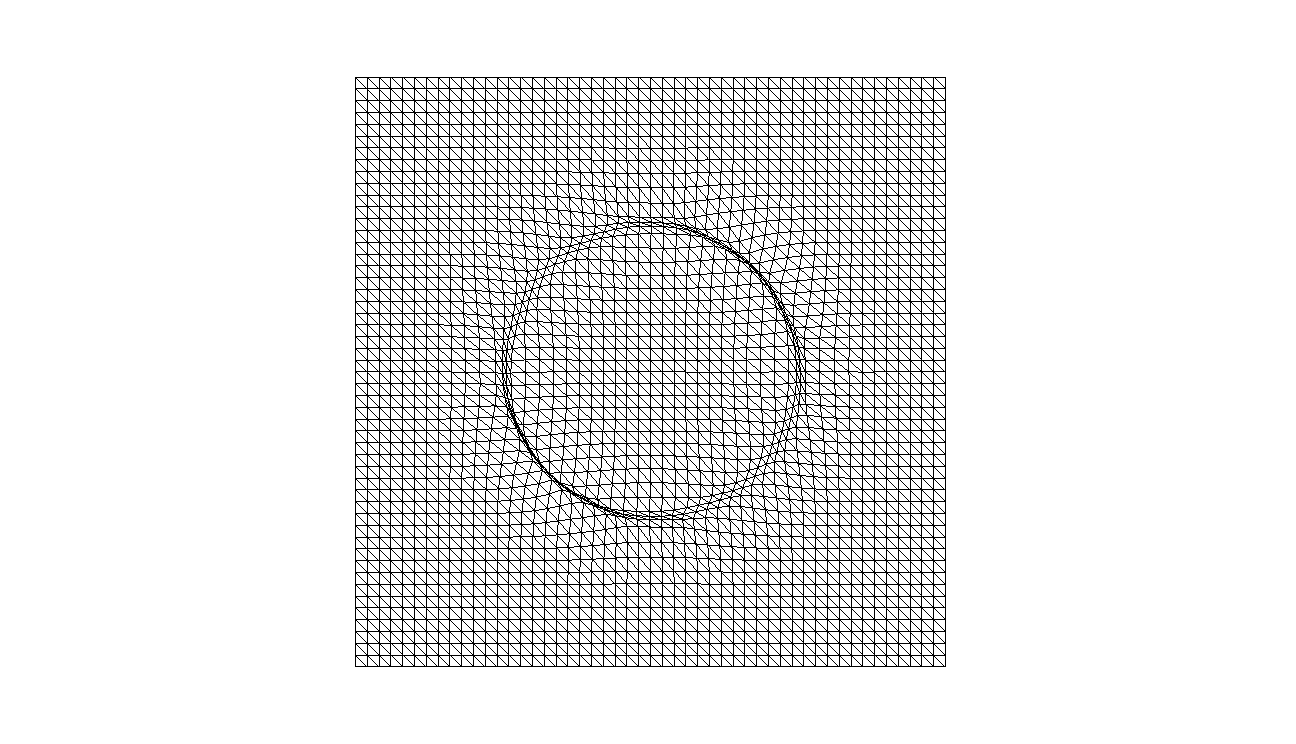
\includegraphics[clip=true, trim = 10cm 0 10cm 0, scale=.25]{Bordeaux/figures/LSadapt.png}
		\captionof{subfigure}{Maillage adapté à la fonction Level Set}
	\end{minipage}
	\captionof{figure}{Exemple d'adaptation à la fonction Level Set \label{fig:exLS}}
\endgroup

\subsection{Construction de la fonction à adapter (avec \(\omega\) donné par l'expression \eqref{eq:omega2})}

\indent Le calcul de \(\omega\) à partir de l'expression \eqref{eq:omega2} est fait en utilisant le gradient et le hessien de la fonction à adapter. Pourtant, dans le cas de la fonction Level Set, l'adaptation n'est pas faite en considérant \(u=LS\), parce qu'on n'a pas de forts gradients, en tenant compte de la lisseté de cette fonction. Ainsi, \(\omega\) ne serait pas capable d'exprimer le raffinement désiré dans chaque partie du maillage. De cette façon, à partir de la fonction Level Set, on a construit une nouvelle fonction qui ait un très fort gradient sur les bords de l'objet.

\indent Idéalement, on construirait une fonction avec un saut, valant \(1\) à l'extérieur et \(-1\) à l'intérieur de l'objet, ce que fournit des très bons raffinements sur la ligne de niveau 0 de la fonction Level Set. Néanmoins, dans la résolution numérique de problèmes de la mécanique des fluides, il est intéressant d'avoir aussi un bon raffinement du maillage sur une couche autour de la surface (la couche limite de l'écoulement), où l'interaction fluide-objet n'est pas négligeable. En effet, pour avoir un calcul précis, un maillage approprié sur la couche limite est requis par la plupart des schémas numériques et logiciels pour les problèmes de fluides \cite{loseille}. Ainsi, on cherche une fonction plus lisse.

\indent Dans un premier moment, on a défini une fonction avec une variation linéaire entre les deux étages (figure \ref{fig:atan}). Néanmoins, les tests réalisés ont fourni des résultats de mauvaise qualité : étant le gradient constant à l'intérieur de la pente, les points dans cette région (y compris les points les proches du bord de l'objet) n'ont pas la tendance de bouger, au contraire des points proches des bordes de la pente, dû à la discontinuité du gradient de \(u\). Par conséquent, l'adaptation produit une maillage avec deux petites couches raffinées, qui ne représentaient pas la surface de l'objet (figure \ref{fig:LSlin}).

\indent

\begingroup
  \centering
  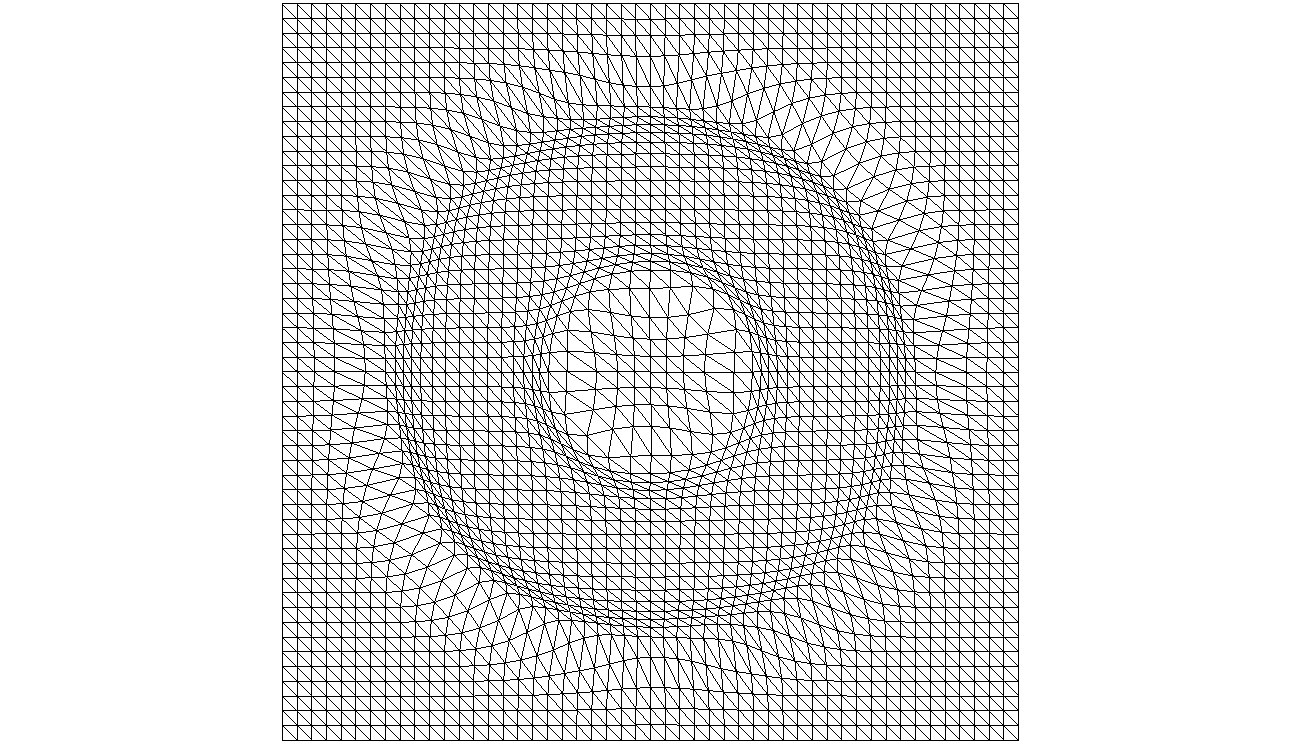
\includegraphics[clip=true, trim = 10cm 0 10cm 0, scale=.22]{Bordeaux/figures/LSlin.png}
  \captionof{figure}{Adaptation à une fonction Level Set modifié avec une variation linéaire \label{fig:LSlin}}
\endgroup

\indent

\indent On a ainsi cherché une fonction dont le gradient est plus variable et continue afin de réduire cet effet. On a obtenu des bons résultats en utilisant

\begin{equation}
	\label{eq:atan}
	u(\vecx) = \frac{1}{1.1.107} atan \left(\frac{2LS(\vecx)}{\delta} \right)
\end{equation}

\noindent étant \(2\delta\) la taille de la couche, choisie par l'utilisateur. Cette fonction est représentée dans la figure \ref{fig:atan}.

\indent

\begingroup
  \centering
  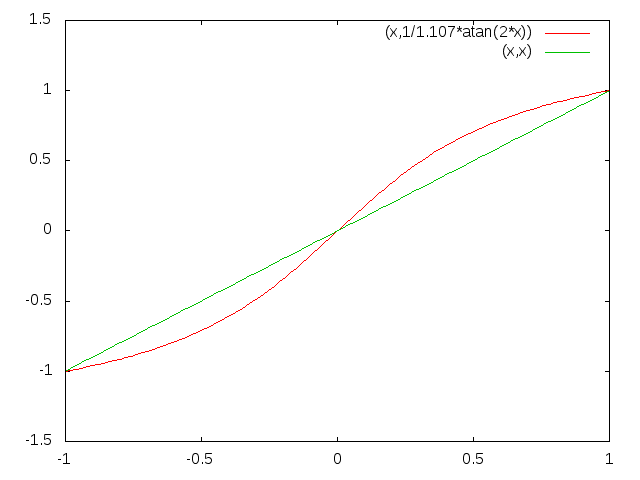
\includegraphics[scale=.4]{Bordeaux/figures/atan.png}
  \captionof{figure}{Comparaison des options pour la lissage de la fonction à adapter   \label{fig:atan}}
\endgroup

\indent

\indent On peut jouer aussi avec le paramètre multiplicateur de \(LS(\vecx)/\delta\) à l'intérieur de la fonction tangent. Avec 1, par exemple, on obtient un résultat plus proche de la pente linéaire; avec 5 ou 10, la fonction devient plus discontinue et la couche de raffinement est plus petite. On reste ainsi avec l'option donnée par \eqref{eq:atan}.



\subsubsection{Choix des paramètres}

\indent Afin de chercher les paramètres qui génèrent le meilleur maillage, plusieurs tests on été réalisés : 

\begin{itemize}
	\item Cas test (objet cible): 
	\begin{itemize}
		\item Cercle;
		\item Triangle;
		\item Profil d'une aile (NACA)
	\end{itemize}
	\item Type de maillage
	\begin{itemize}
		\item Structuré;
		\item Non structuré
	\end{itemize}
\end{itemize}

\indent Les meilleurs maillages obtenus on été utilisés pour résoudre un problème d'écoulement autour de l'objet, afin de vérifier l'influence sur les résultats. Les conclusions des tests sont les suivants : 

\begin{itemize}
  \item Pour le calcul de \(\omega\), il faut plutôt utiliser le gradient de \(u\). Le hessien peut être aussi utilisé, mais il a la tendance de créer deux couches raffinées dans les bords de la région de variation de la fonction \(u\) (figure \ref{fig:alphabeta});
  \item Le raffinement d'une certaine région du maillage cause un étirement dans la direction normale à surface des éléments voisins à cette région. Ce résultat n'est pas désirable car on veut plutôt une anisotropie dans la direction de l'écoulement du fluide (figure \ref{fig:anisoNormal}) : l'erreur d'interpolation est plus petit si on a des triangles anisotropes dont le côté le plus long est dans la direction des petites dérivées de deuxième ordre de la solution \cite{rippa}. Ainsi, il est important de avoir une valeur de \(\delta\) assez grande.
  \item Néanmoins, \(\delta\) ne peut être trop grand, car la fonction arctangente s'approche de la pente linéaire, et on n'obtient pas un bon raffinement à l'intérieur de la couche.
\end{itemize}


\begingroup
	\begin{minipage}[t]{.5\linewidth}
		\centering
		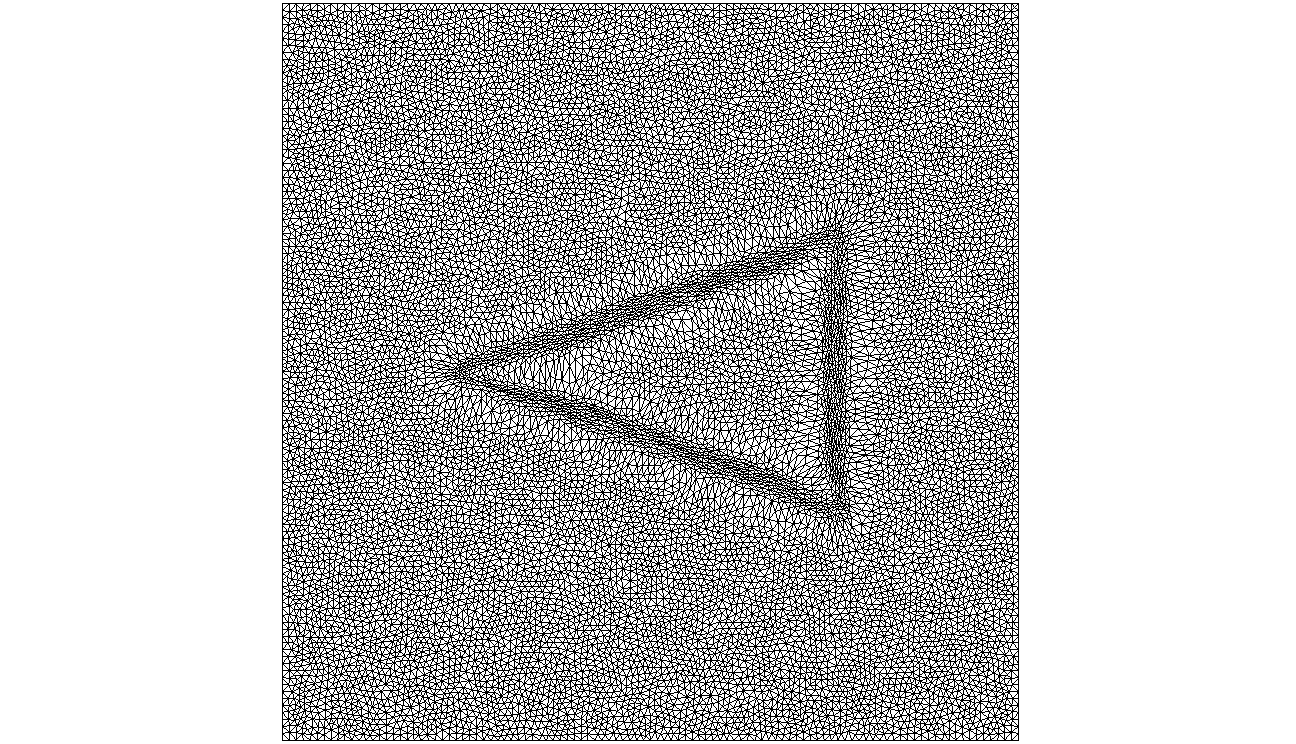
\includegraphics[clip=true, trim = 10cm 0 10cm 0, scale=.25]{Bordeaux/figures/alphabeta0.png}
		\captionof{subfigure}{\(\alpha = 1000, \beta = 0\)}
	\end{minipage}
	\hfill
	\begin{minipage}[t]{.5\linewidth}
		\centering
		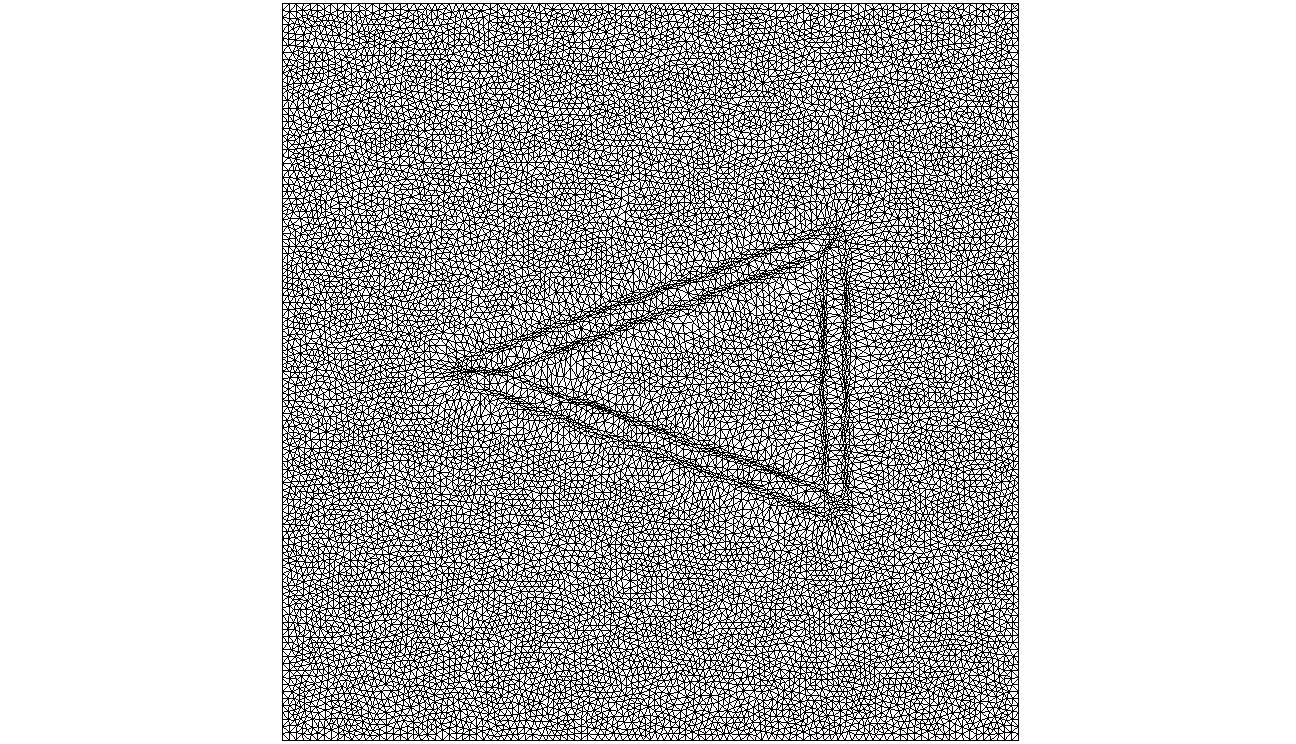
\includegraphics[clip=true, trim = 10cm 0 10cm 0, scale=.25]{Bordeaux/figures/alphabeta1.png}
		\captionof{subfigure}{\(\alpha = 0, \beta = 1000\)}
	\end{minipage}
	\captionof{figure}{Influence des paramètres \(\alpha\) et \(\beta\) sur l'adaptation du maillage (\(\delta = 0.02\)) \label{fig:alphabeta}}
\endgroup

\begingroup
	\centering
	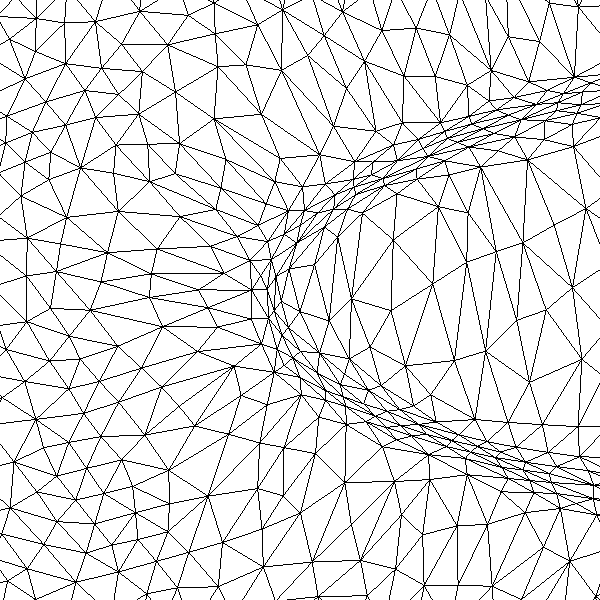
\includegraphics[scale=.25]{Bordeaux/figures/anisoNormal.png}
	\captionof{figure}{Détail d'un maillage obtenu avec \(\delta = 0.005\) \label{fig:anisoNormal}}
\endgroup

\indent

\indent En tenant compte de ces conclusions, on recommande l'utilisation des paramètres suivants (on rappelle qu'on utilise toujours les normes du gradient et du hessien normalisés entre 0 et 1) : 

\begin{equation*}
	\boldsymbol{\alpha} = 1000, \qquad 
	\boldsymbol{\beta} = 0, \qquad
	\boldsymbol{\delta} = 0.01,\  0.02
\end{equation*}

\indent On peut aussi faire des adaptations successives, en faisant varier les paramètres, afin d'obtenir d'autres résultats. Par exemple, on peut faire une première adaptation avec \(\delta = 0.02\) pour obtenir une bonne couche raffinée, et après une deuxième avec \(\delta = 0.01\) pour obtenir un raffinement plus précis autour de la surface. 

\indent La figure \ref{fig:example} présente quelques exemples d'adaptation à une fonction Level Set, avec les paramètres présentés ci-dessus, sur un maillage non structuré avec environ 28000 noeuds : 

\begingroup
	\begin{minipage}[t]{.5\linewidth}
    		\centering
		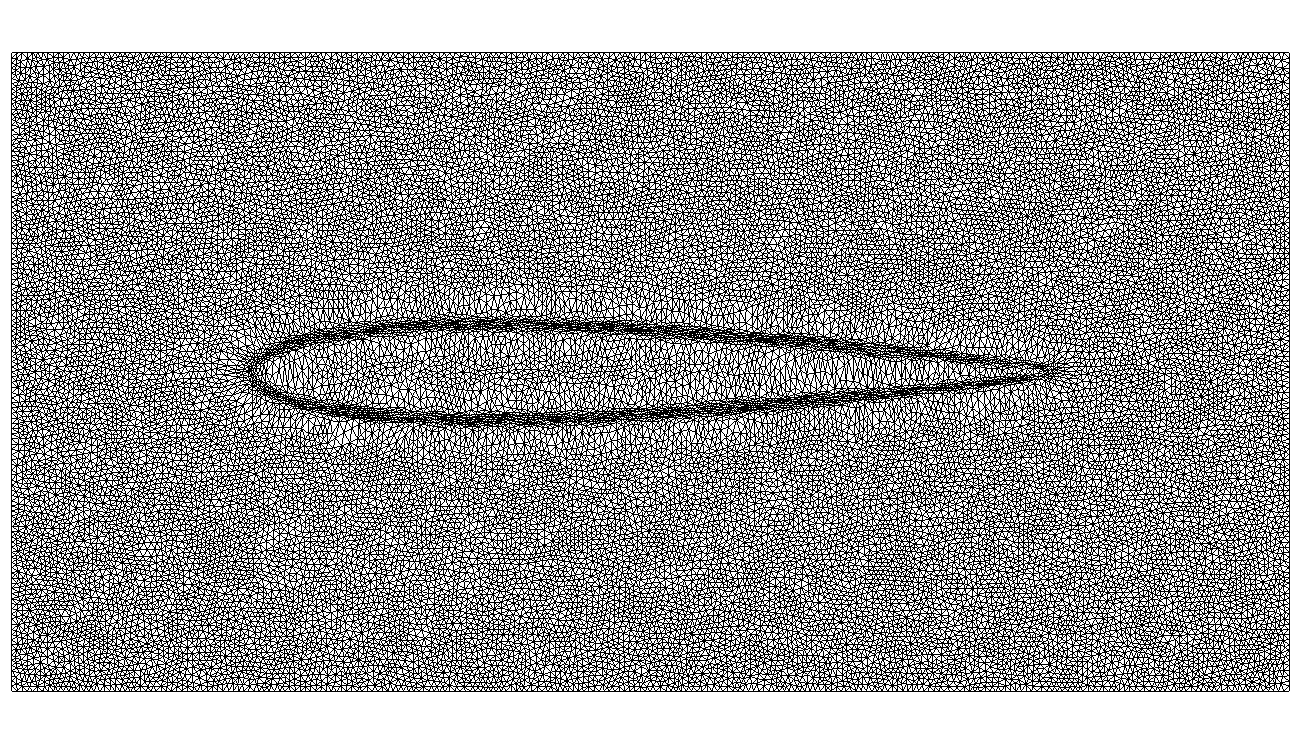
\includegraphics[scale=.15]{{Bordeaux/figures/example1}.png}
		\captionof{subfigure}{\(\delta = 0.01\)}
  	\end{minipage}
	\begin{minipage}[t]{.5\linewidth}
    		\centering
		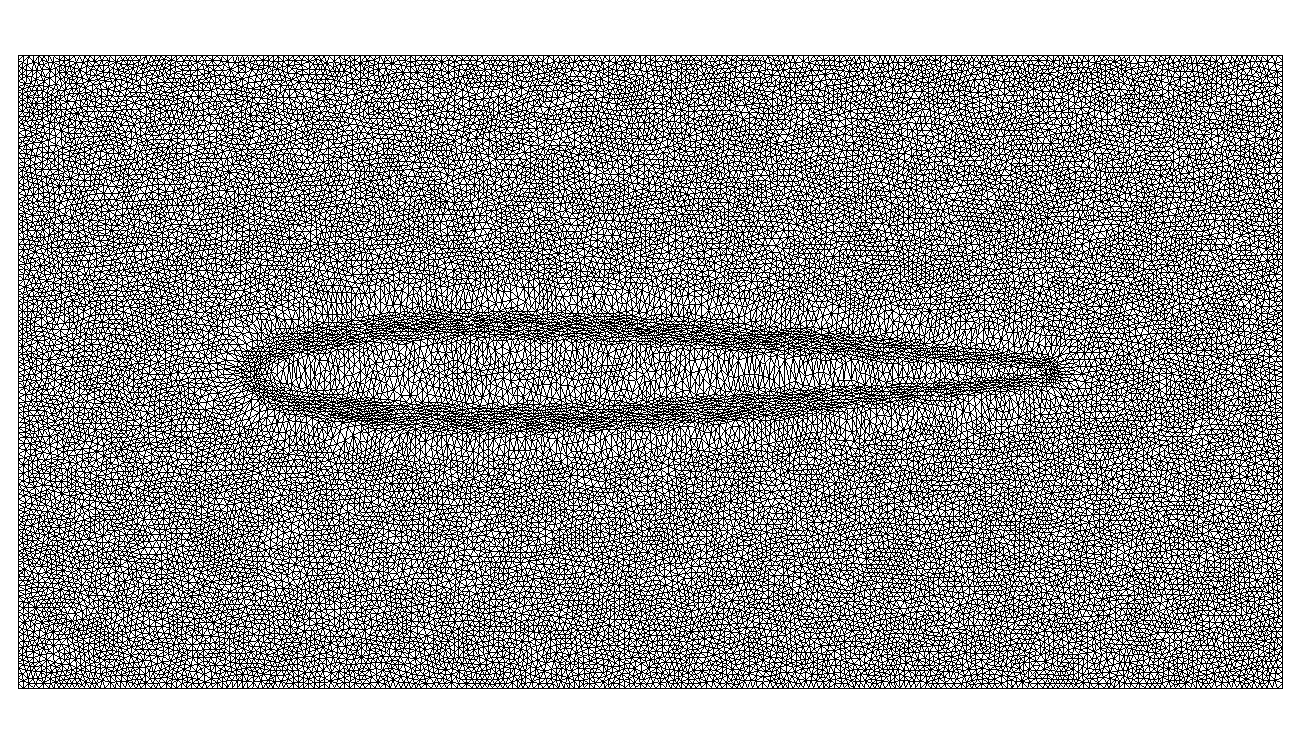
\includegraphics[scale=.15]{{Bordeaux/figures/example2}.png}
		\captionof{subfigure}{\(\delta = 0.02\)}
  	\end{minipage}
  	\captionof{figure}{Exemples d'adaptation à une fonction Level Set \label{fig:example}}
\endgroup


\subsection{Calcul des tailles désirées}

\indent Le calcul des tailles désirées est basée sur la définition d'une métrique pour chaque point du maillage. Elle s'agit d'une matrice \(2 \times 2\) (dans le cas bidimensionnel) définie positive symétrique, construite de façon a contrôler l'erreur de la représentation de la solution sur le maillage modifié \cite{leo}.

\indent La description détaillée de la définition, calcul et interprétation géométrique de la métrique seront faites dans la section \ref{sec:adapPhysique}, pour l'adaptation à une solution physique. Dans le cas de l'adaptation Level Set, on a implémenté un calcul simple des tailles désirées, en se basant sur la méthode utilisée par \cite{ducrot}, qui permet de contrôler la distance de Hausdorff entre la surface de l'objet et sa représentation. En faisant attention toujours à l'importance, pour une bonne adaptation,  de créer une fonction \(\omega\) qui soit au même temps assez lisse et qui présente des variations qui permettent le mouvement des noeuds, on définit, avec le paramètre \(\delta\), des couches pour l'imposition des tailles : 

\begin{equation*}
	\hdes (\vecx_i) =
	\begin{cases}
		\hm \ \ \ si \ \ |LS(\vecx_i)| \leq \frac{\delta}{2} \\
		2\hm \ \ \ si \ \ \frac{\delta}{2} \leq |LS(\vecx_i)|  \leq \delta \\
		\hM \ \ \ sinon
	\end{cases}
\end{equation*}

\noindent et on lisse les tailles sur le maillage avec le logiciel \emph{MMG}, en imposant une gradation de 10\%.

\subsubsection{Résultats}

\indent La figure \ref{fig:adaptMet} illustre l'adaptation Level Set basée sur l'imposition de tailles désirées à chaque noeud.

\begingroup
	\begin{minipage}[t]{.5\linewidth}
		\centering
		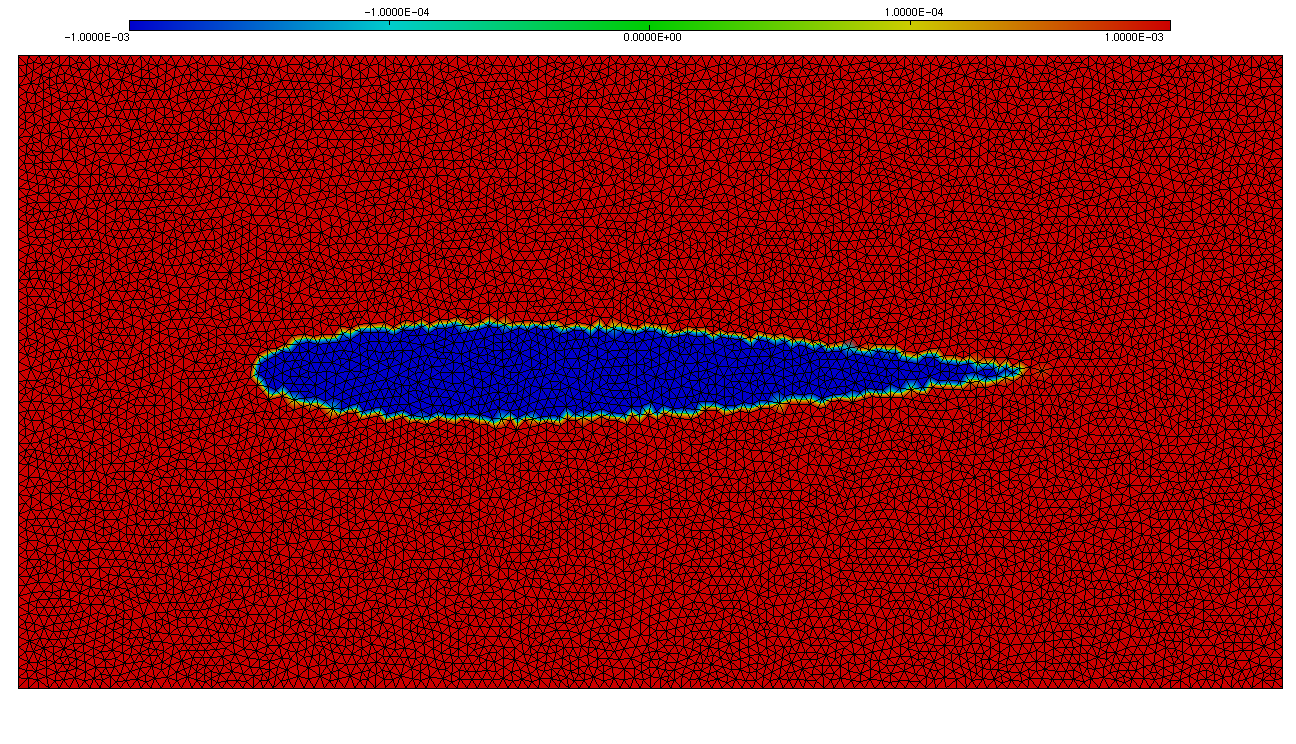
\includegraphics[scale=.15]{Bordeaux/figures/metLSNacaLS.png}
		\captionof{subfigure}{Fonction Level Set}
	\end{minipage}
	\hfill
	\begin{minipage}[t]{.5\linewidth}
		\centering
		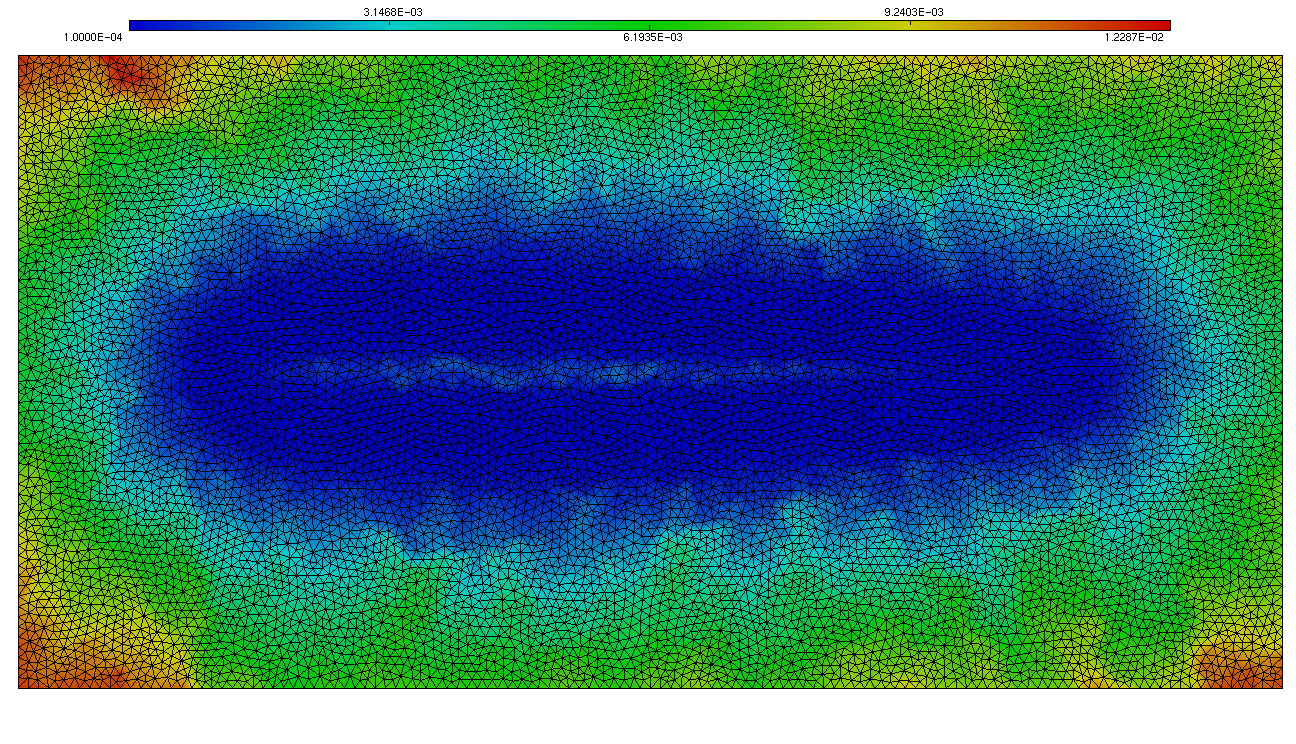
\includegraphics[scale=.15]{Bordeaux/figures/metLSNacaMet.png}
		\captionof{subfigure}{Tailles désirées}
	\end{minipage}	
	\begin{minipage}[t]{1.\linewidth}
		\centering
		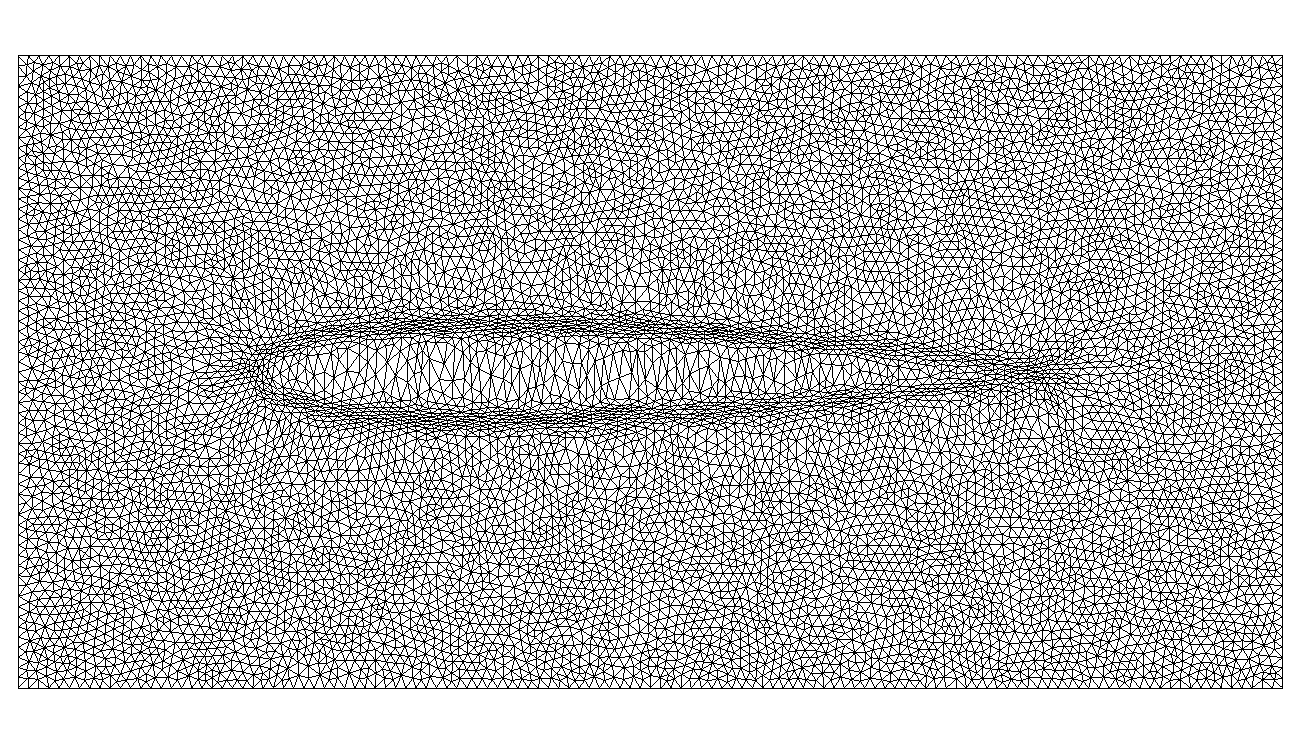
\includegraphics[scale=.2]{Bordeaux/figures/metLSNacaAdapt.png}
		\captionof{subfigure}{Maillage adapté (20 itérations)}
	\end{minipage}	
	\captionof{figure}{Adaptation à une fonction Level Set à partir de l'imposition des tailles désirées \label{fig:adaptMet}}
\endgroup

\indent

\indent En réalisant des tests comme ceux présentés dans la figure \ref{fig:adaptMet}, on a bien validé la procédure d'adaptation utilisant les tailles désirées pour définir la fonction $\omega$. Ainsi, à partir de cette validation, on n'a utilisé que ce nouveaux modèle dans notre procédure, parce qu'il est plus simple et beaucoup plus accessible à l'utilisateur final de la bibliothèque, qui n'est pas forcement habitué aus détails concernant l'adaptation de maillage. Pour cet utilisateur, c'est plus naturel définir des tailles $h_{min}$ et $h_{max}$ (qui ont une interprétation physique évidente et indépendante du problème considéré) que définir des coefficients $\alpha$ et $\beta$ (que en plus dépendent du problème). 


\subsection{Relaxation et qualité du maillage}

\indent Pendant la résolution du système linéaire, on fait, si nécessaire, une relaxation des déplacements calculés afin d'éviter le croisement des noeuds et la conséquente occurrence d'aires négatives. Néanmoins, en dépendant du maillage de départ (par exemple, un maillage déjà raffiné), la relaxation est trop contraignante et impose l'arrêt de l'algorithme lors des premières itérations, ce qui peut être provoqué par un petit nombre d'éléments.

\indent On a ainsi implémenté, dans les premières itérations, un prétraitement d'optimisation, selon le schéma suivant :

\begin{itemize}
  \item Si le numéro de l'itération actuelle n'est pas supérieur à \(iter_{optim}\) : 
  \begin{enumerate}
    \item Identifier tous les éléments qui demanderont de la relaxation;
    \item Classifier ces éléments selon un critère de qualité (mesure de l'anisotropie);
    \item Optimiser les \(n_{optim}\) éléments les plus critiques de cette liste
  \end{enumerate}   
\end{itemize}

\indent L'optimisation réalisée consiste en, itérativement, approcher chaque noeud \(i\) de l'élément concerné du barycentre des noeuds voisins de \(i\). L'optimisation est arrêtée dès qu'aucun des trois noeuds de l'élément bouge au dessus d'un seuil, ou qu'au moins un des noeuds n'arrive pas à réduire l'anisotropie au dessous d'une certaine pourcentage, par rapport au début de l'itération.

\indent La figure \ref{fig:optim} montre le résultat de son application sur un élément : 

\indent

\begingroup
	\begin{minipage}[t]{.5\linewidth}
    		\centering
		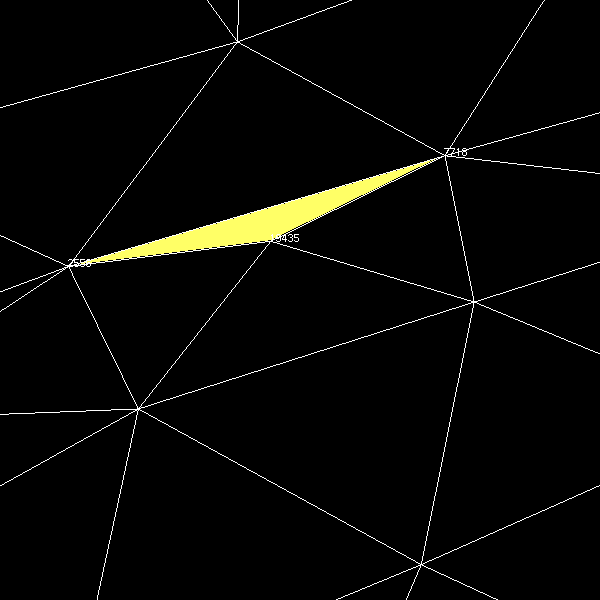
\includegraphics[scale=.25]{{Bordeaux/figures/optim_avant}.png}
		\captionof{subfigure}{Avant l'optimisation}
  	\end{minipage}
  	\hfill
	\begin{minipage}[t]{.5\linewidth}
    		\centering
		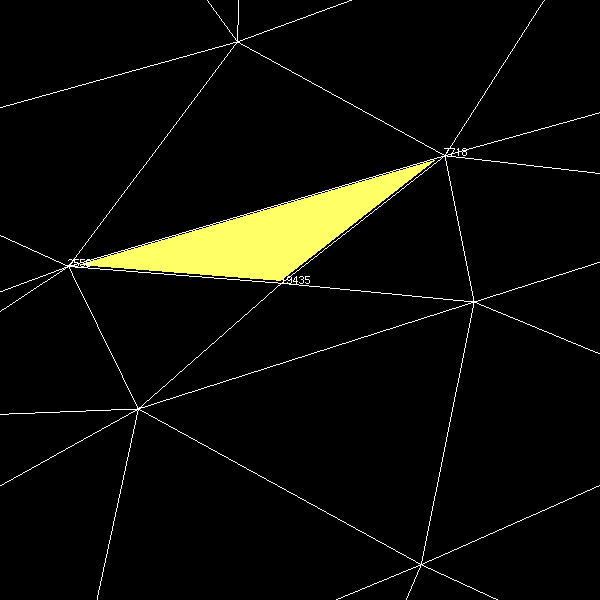
\includegraphics[scale=.25]{{Bordeaux/figures/optim_apres}.png}
		\captionof{subfigure}{Après l'optimisation}
  	\end{minipage}
  	\captionof{figure}{Résultat de l'optimisation d'un élément \label{fig:optim}}
\endgroup

\indent

\indent Pour que le prétraitement ne soit pas très coûteux, on a choisi \(n_{optim} = 10\) e \(iter_{optim} = 2\). Les tests réalisés montrent des très bons résultats quand l'adaptation s'arrête au début de l'exécution, dû à la présence d'éléments très anisotropes au début, et avec l'optimisation on arrive à tourner toutes les itérations. Néanmoins, si appliqué sur un maillage de bonne qualité et qui ne demande pas une forte relaxation, les gains sont en général petits (ou même on perd un peu de la qualité du résultat final).


\subsection{Adaptation 3D}

\indent Après le développement et validation du modèle bidimensionnel décrit jusqu'ici, avec l'obtention de bons résultats d'adaptation des maillages, on l'a étendu au cas tridimensionnel. Du point de vue théorique, cette extension est assez simple, étant le modèle toujours décrit par le problème \eqref{eq:systeme}. Le développement de sa formulation faible reste aussi la même, et on se ramène ainsi à la résolution des systèmes linéaires

\begin{equation*}
	\begin{cases}
		Kx = 0 \\
		Ky = 0 \\
		Kz = 0
	\end{cases}
\end{equation*}

\indent Comme ces systèmes sont indépendants et ont la même forme, l'extension du cas 2D au 3D a été également simple du point de vue de l'implémentation. En effet, parmi les calculs décrits en détail dans les sous-sections \ref{subsec:calculK} et \ref{subsec:jacobi}, l'unique modification concerne le calcul des vecteurs normaux (\((\nabref \phii)^T = \frac{\normT{i}}{d\text{!}|T|}\), avec \(d=3\)). Ainsi, les éléments de la matrice \(K\) sont donnés par


\begin{equation*}
\begin{gathered}
\begin{aligned}
	k_{ij} & = \iDomh{ \omega \nabref \phii  \cdot \nabref \phij } = \sum_{T \ni i} {\iT{ \omega \nabref \phii \cdot \nabref \phij }} = \\
	       &  = \sum_{T \ni i}
	              { 
	                     { |T|\omega^T \frac{\normT{i}\cdot \normT{j}}{(3\text{!}|T|)^2}
	                     }
	              }
	          = \sum_{T \ni i}
	              { 
	                     { \omega^T \frac{\normT{i}\cdot \normT{j}}{36|T|}
	                     }
	              }	              
\end{aligned}
\end{gathered}
\end{equation*}

\indent On présente dans les figures \ref{fig:adaptSphere} à \ref{fig:adaptHole} quelques résultats de l'adaptation Level Set tridimensionnelle, à partir de l'imposition des tailles désirées. Les fonctions Level Set utilisées sont celles de la figure \ref{fig:LS}. Malgré les résultats analogues au cas 2D et cohérents avec les objectifs ici proposés, l'adaptation 3D a des limitations plus fortes concernant le nombre de points du maillage, qui peut devenir très grande pour qu'on ait un maillage suffisamment fine pour la bonne représentation de la fonction Level Set, et la relaxation de l'adaptation, puisque le dégrée de liberté additionnel peut conduire plus rapidement au croisement des noeuds.

\indent Les domaines de départ sont plus raffinées dans les régions où se trouve l'objet, afin de minimiser l'influence des bords sur l'adaptation. Le logiciel \emph{MMG} a été utilisé pour les générer, en imposant une taille minimale \(hmin =  0.05\) et une gradation de \(hgrad = 1.1\) de la variation de las tailles. Les adaptations ont été faites avec \(\delta\) entre 0.05 et 0.07.

\indent

\begingroup
	\begin{minipage}{.3\linewidth}
		\centering
		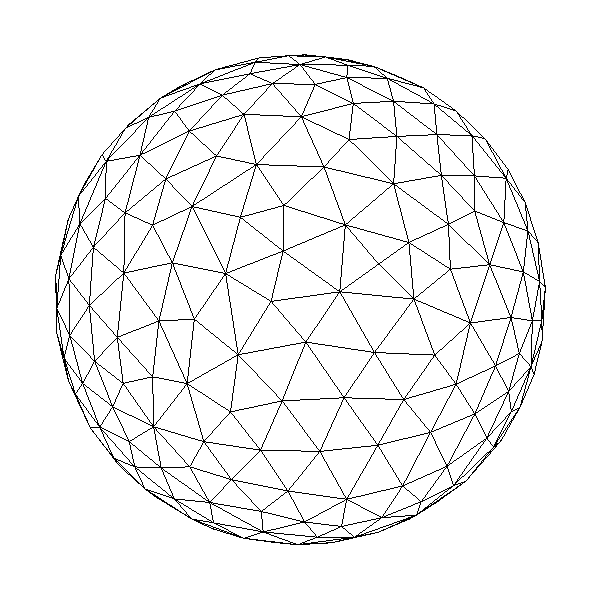
\includegraphics[scale=.2]{Bordeaux/figures/3D/sphereLS.png}
		\captionof{subfigure}{Sphere \label{fig:sphereLS}}
	\end{minipage}
	\hfill
	\begin{minipage}{.3\linewidth}
		\centering
		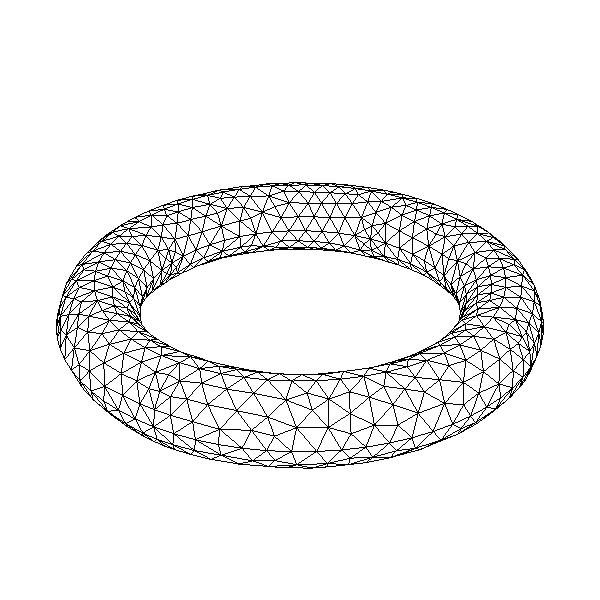
\includegraphics[scale=.2]{Bordeaux/figures/3D/torusLS.png}
		\captionof{subfigure}{Tore \label{fig:torusLS}}
	\end{minipage}
	\hfill
	\begin{minipage}{.3\linewidth}
		\centering
		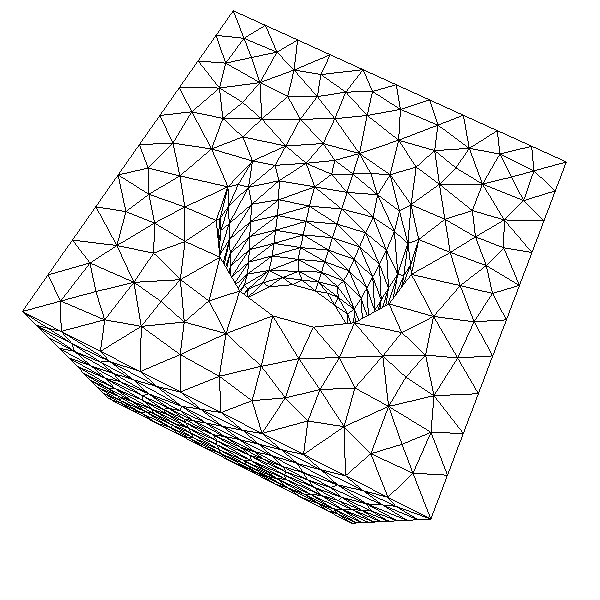
\includegraphics[scale=.2]{Bordeaux/figures/3D/holeLS.png}
		\captionof{subfigure}{Boîte avec un trou \label{fig:holeLS}}
	\end{minipage}
	\captionof{figure}{Fonctions Level Set utilisées \label{fig:LS}}
\endgroup

\indent

\indent

\begingroup
	\begin{minipage}[t]{.5\linewidth}
		\centering
		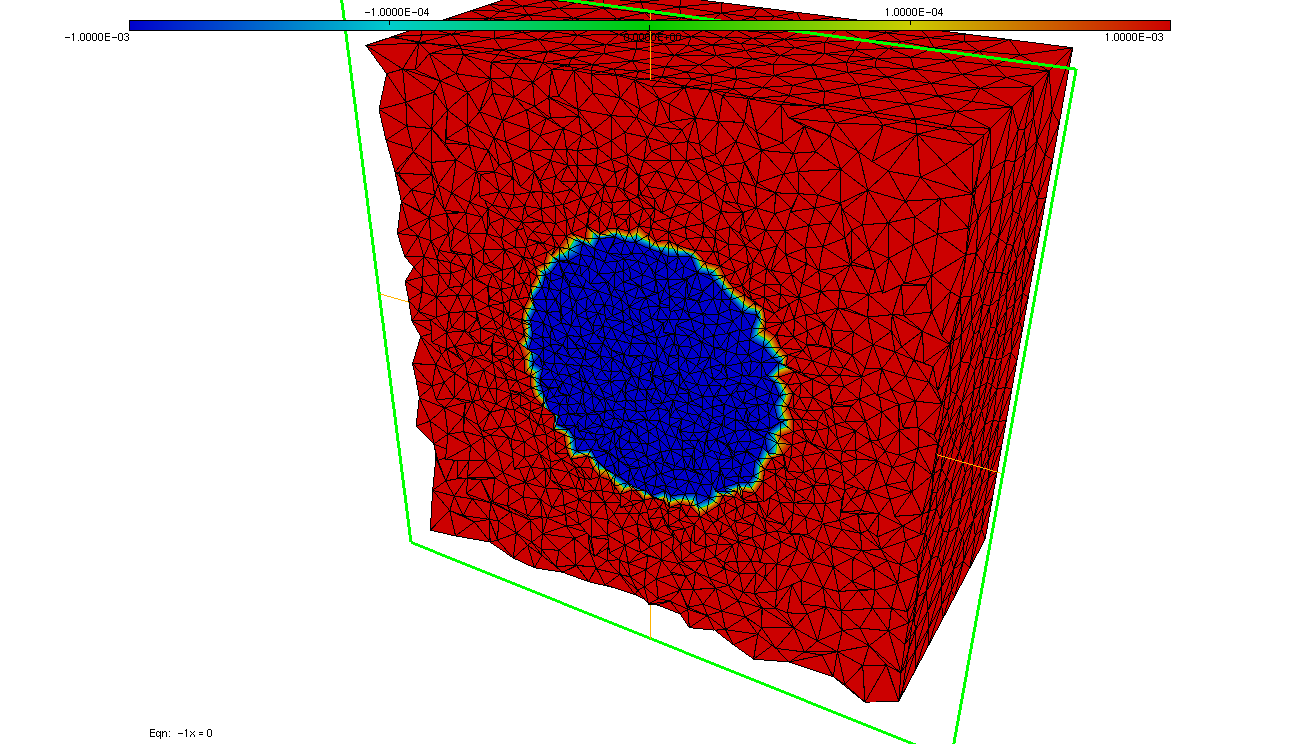
\includegraphics[clip=true, trim=5cm 0 2cm 0, scale=.2]{Bordeaux/figures/3D/sphereDomLS.png}
		\captionof{subfigure}{Fonction Level Set}
	\end{minipage}
	\hfill
	\begin{minipage}[t]{.5\linewidth}
		\centering
		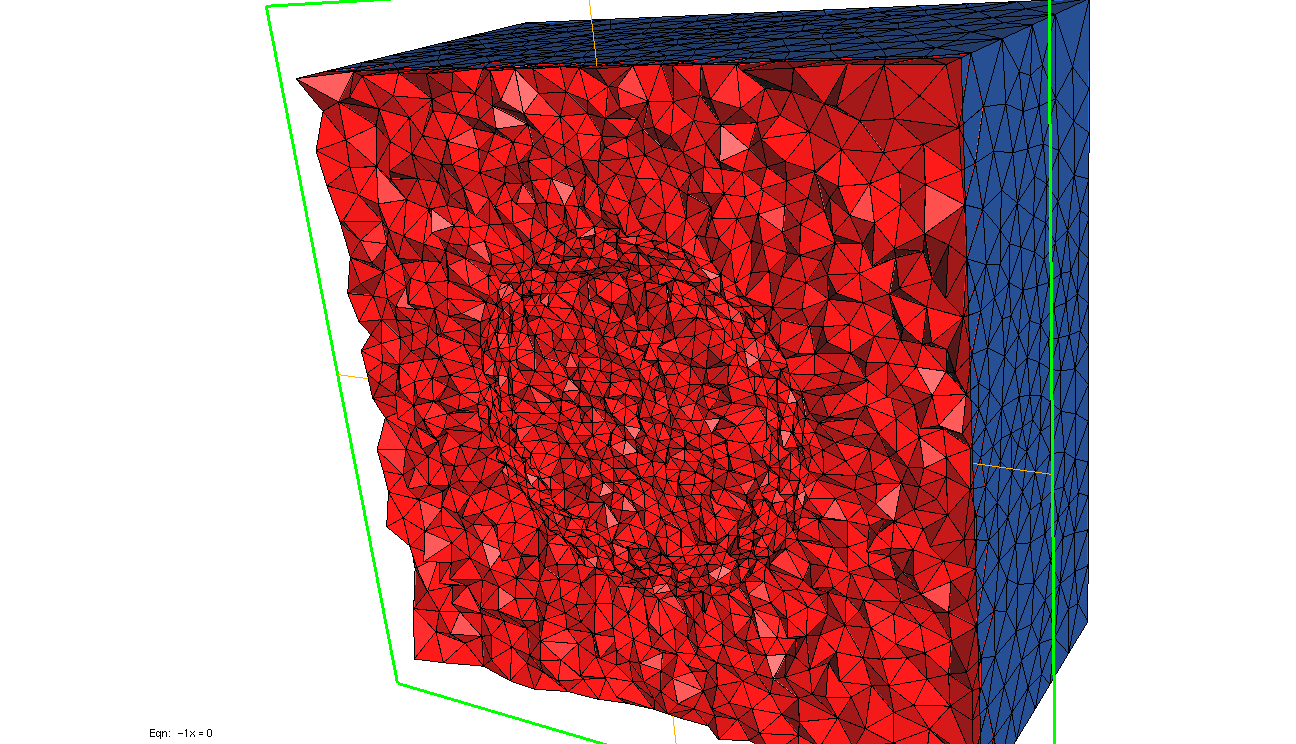
\includegraphics[clip=true, trim=5cm 0 5cm 0, scale=.2]{Bordeaux/figures/3D/sphereAdapt.png}
		\captionof{subfigure}{Maillage adapté (7 itérations)}
	\end{minipage}
	\captionof{figure}{Adaptation du maillage à la sphère (environ 34000 noeuds) \label{fig:adaptSphere}}
\endgroup

\indent

\indent

\begingroup
	\begin{minipage}[t]{.5\linewidth}
		\centering
		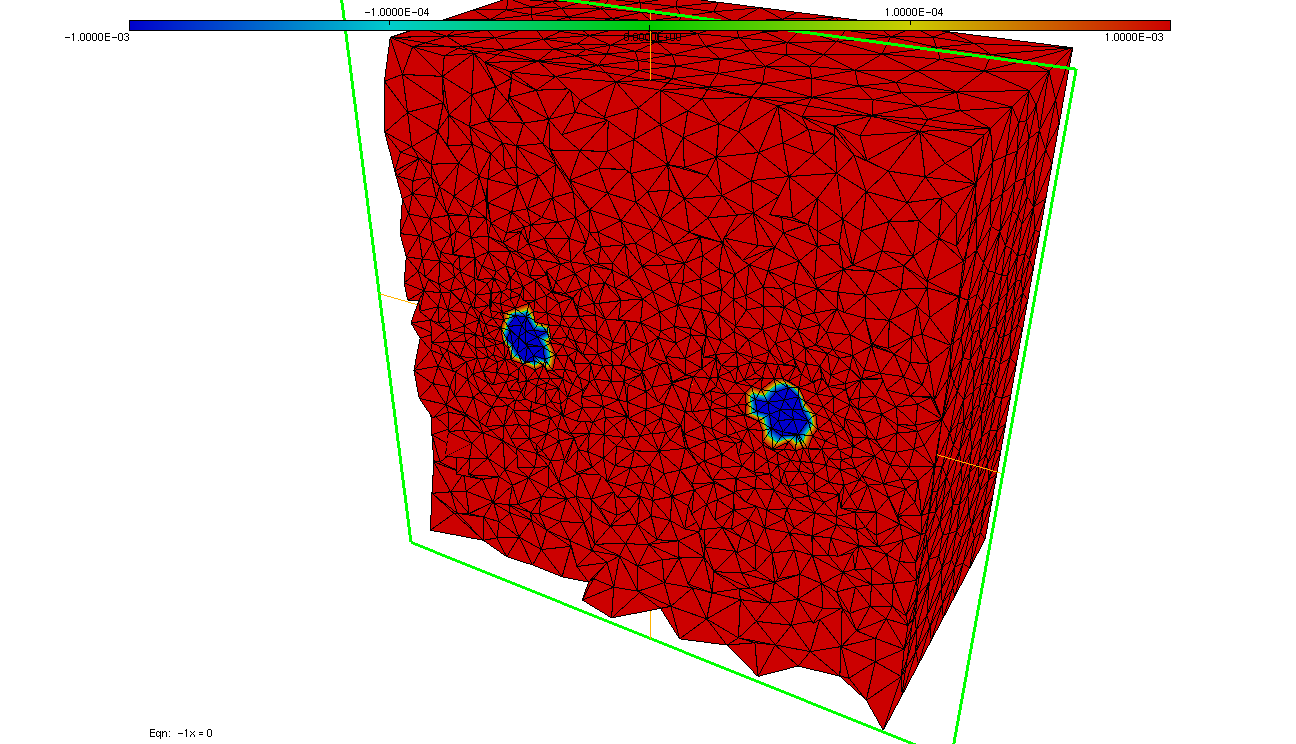
\includegraphics[clip=true, trim=5cm 0 2cm 0, scale=.2]{Bordeaux/figures/3D/torusDomLS1.png}
		\captionof{subfigure}{Fonction Level Set}
	\end{minipage}
	\hfill
	\begin{minipage}[t]{.5\linewidth}
		\centering
		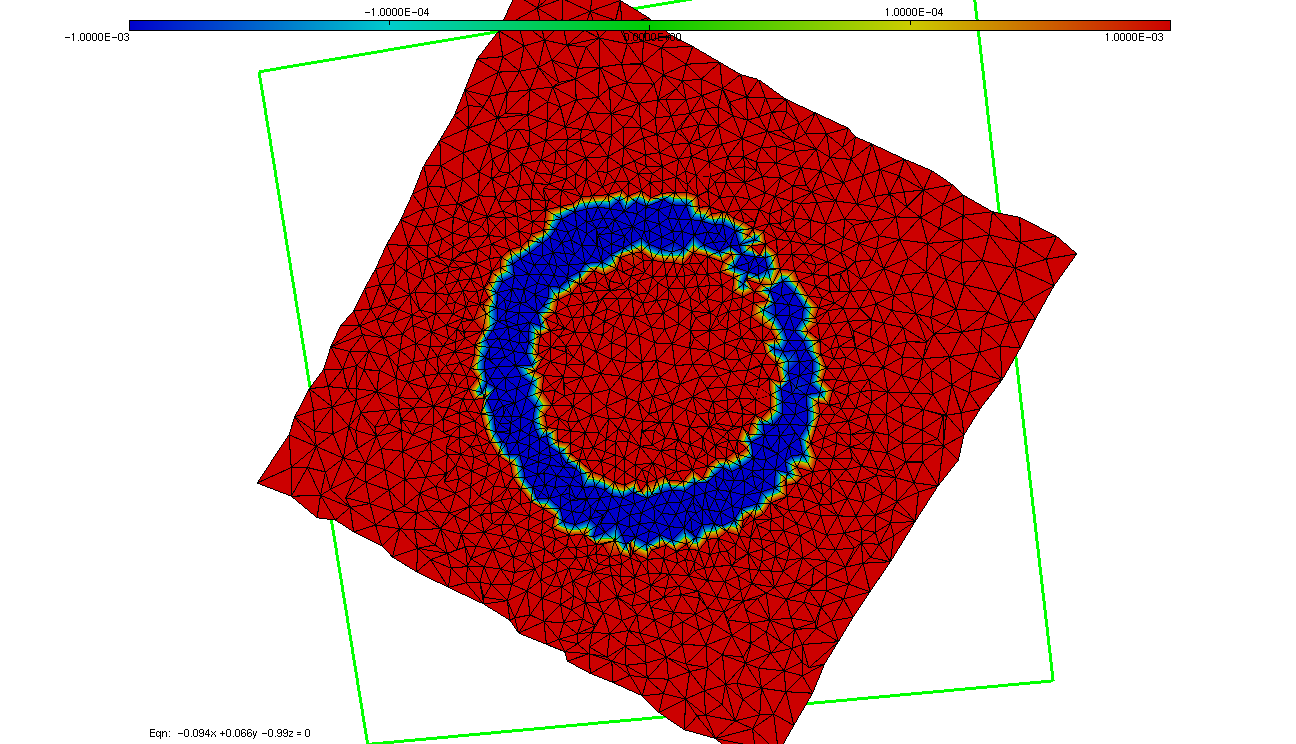
\includegraphics[clip=true, trim=5cm 0 2cm 0, scale=.2]{Bordeaux/figures/3D/torusDomLS2.png}
		\captionof{subfigure}{Fonction Level Set}
	\end{minipage}
	\begin{minipage}[t]{.5\linewidth}
		\centering
		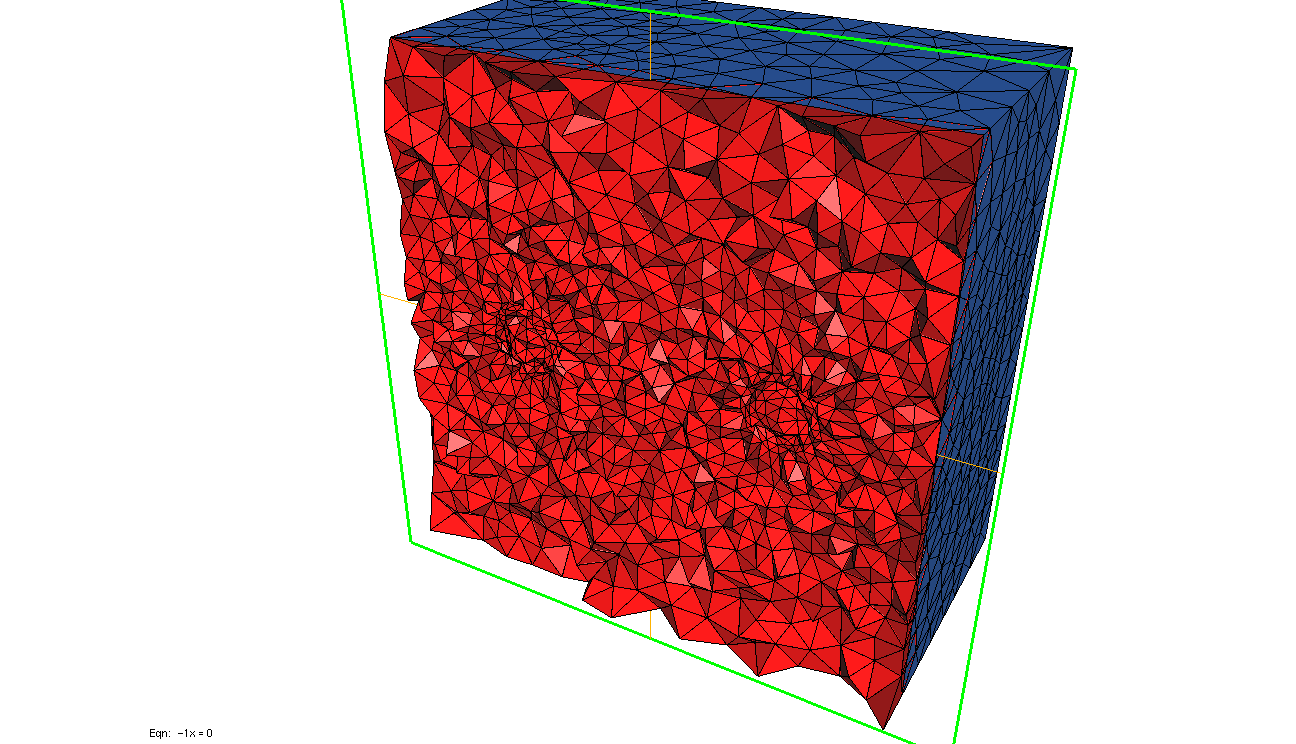
\includegraphics[clip=true, trim=5cm 0 2cm 0, scale=.2]{Bordeaux/figures/3D/torusAdapt2.png}
		\captionof{subfigure}{Maillage adapté (8 itérations)}
	\end{minipage}
	\hfill
	\begin{minipage}[t]{.5\linewidth}
		\centering
		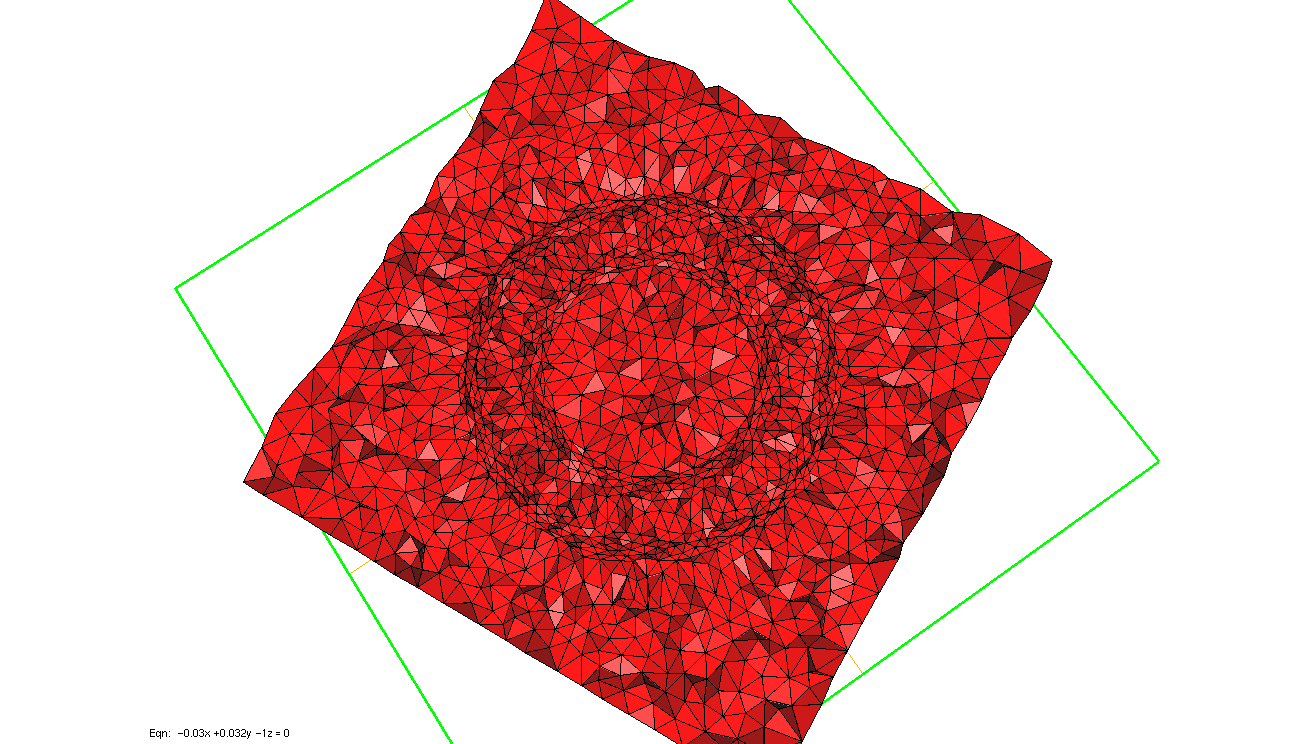
\includegraphics[clip=true, trim=5cm 0 2cm 0, scale=.2]{Bordeaux/figures/3D/torusAdapt1.png}
		\captionof{subfigure}{Maillage adapté (8 itérations)}
	\end{minipage}
	\captionof{figure}{Adaptation du maillage au tore (environ 25000 noeuds) \label{fig:adaptTorus}}
\endgroup

\indent

\indent

\begingroup
	\begin{minipage}[t]{.5\linewidth}
		\centering
		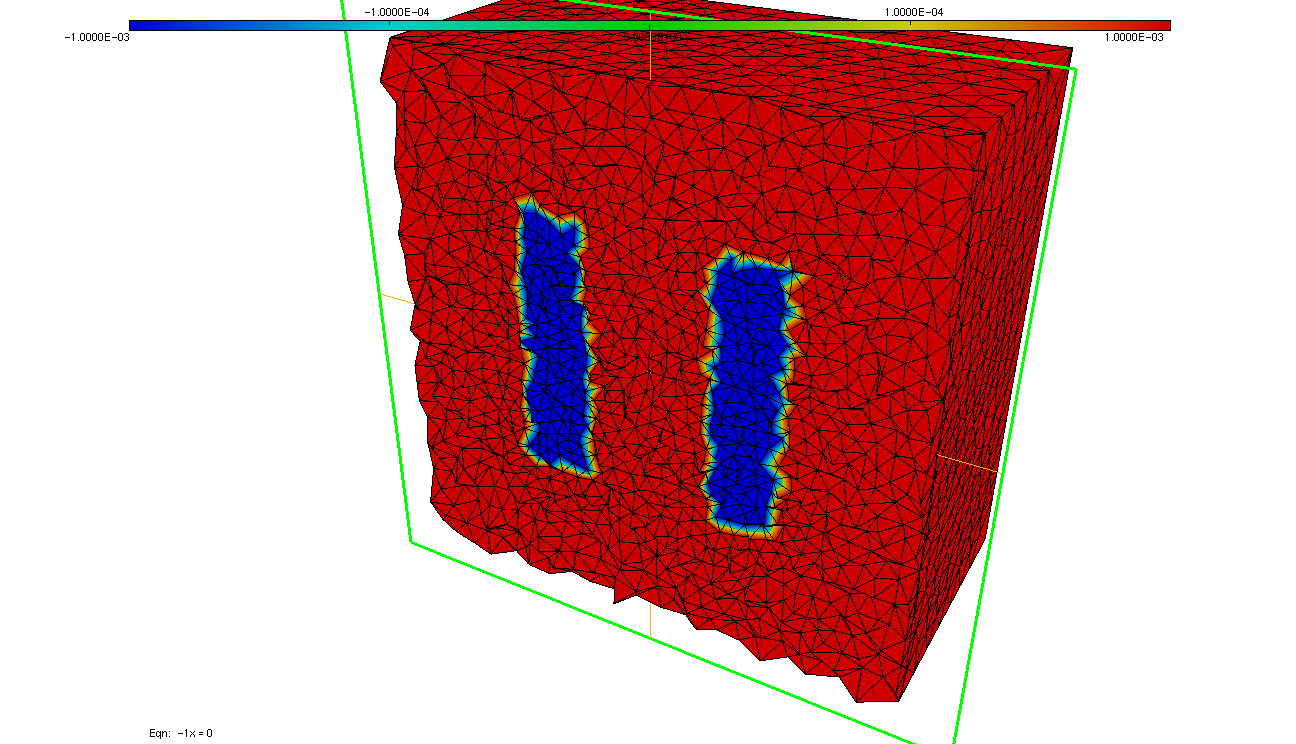
\includegraphics[clip=true, trim=5cm 0 2cm 0, scale=.2]{Bordeaux/figures/3D/holeDomLS1.png}
		\captionof{subfigure}{Fonction Level Set}
	\end{minipage}
	\begin{minipage}[t]{.5\linewidth}
		\centering
		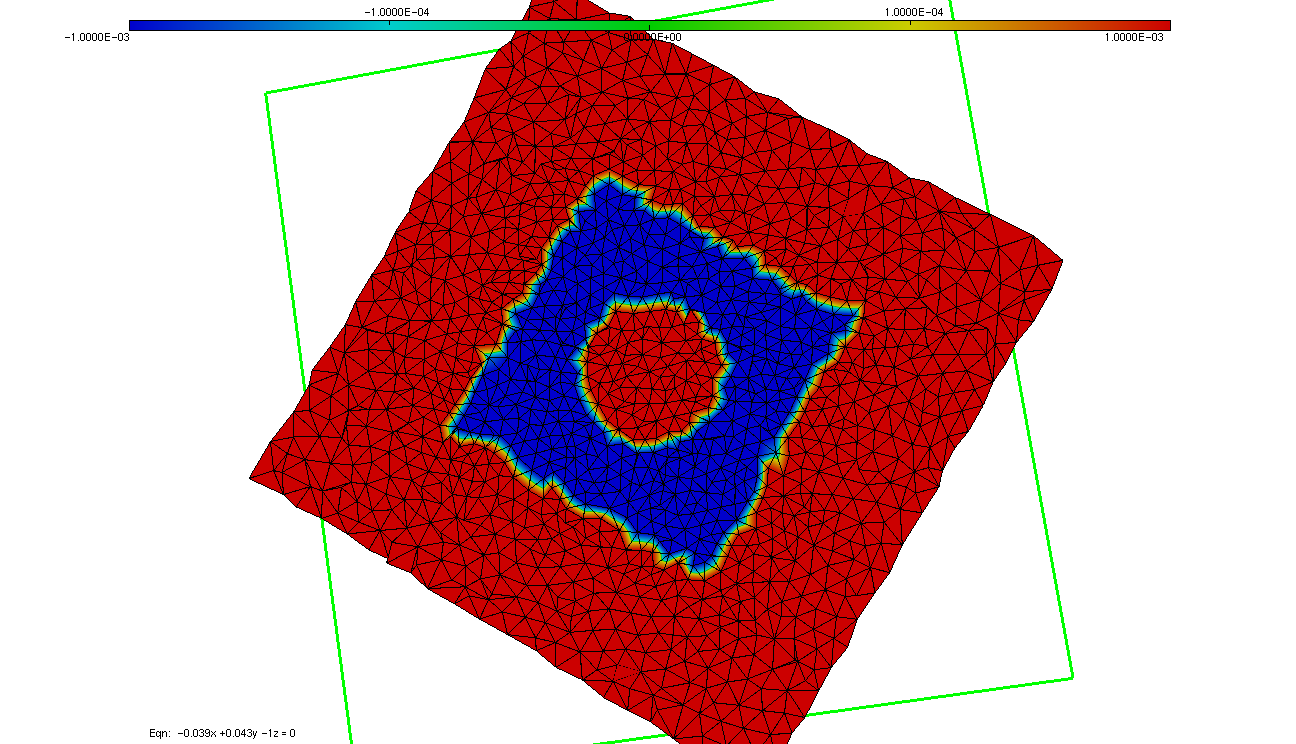
\includegraphics[clip=true, trim=5cm 0 2cm 0, scale=.2]{Bordeaux/figures/3D/holeDomLS2.png}
		\captionof{subfigure}{Fonction Level Set}
	\end{minipage}
	\begin{minipage}[t]{.5\linewidth}
		\centering
		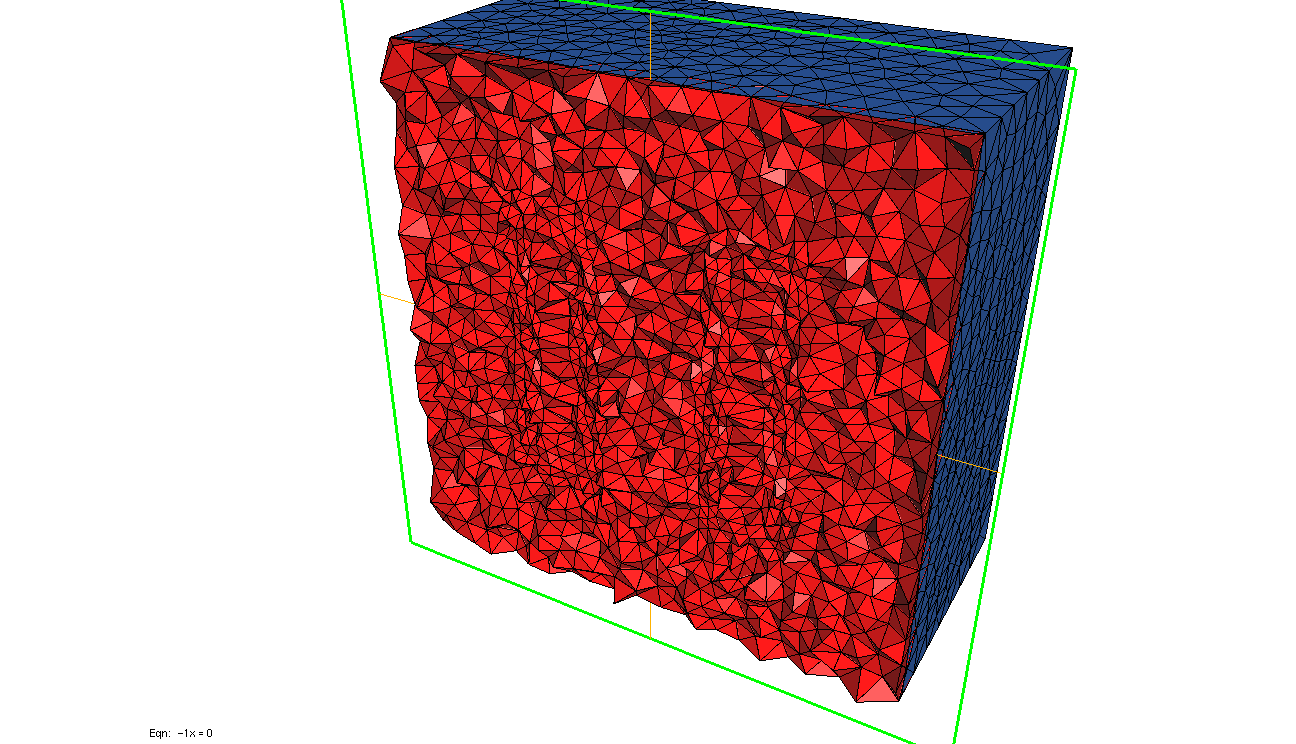
\includegraphics[clip=true, trim=5cm 0 2cm 0, scale=.2]{Bordeaux/figures/3D/holeAdapt1.png}
		\captionof{subfigure}{Maillage adapté (5 itérations)}
	\end{minipage}
	\begin{minipage}[t]{.5\linewidth}
		\centering
		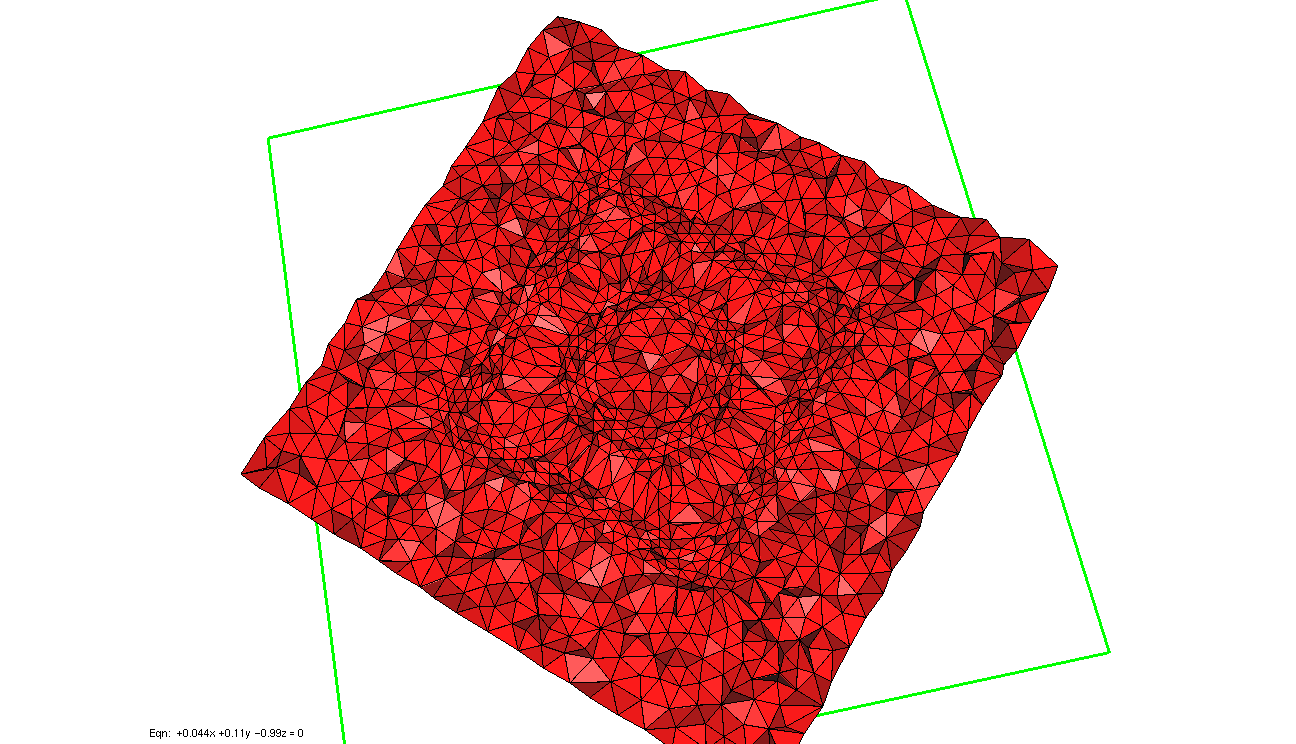
\includegraphics[clip=true, trim=5cm 0 2cm 0, scale=.2]{Bordeaux/figures/3D/holeAdapt2.png}
		\captionof{subfigure}{Maillage adapté (5 itérations)}
	\end{minipage}
	\captionof{figure}{Adaptation du maillage à une boîte avec un trou (environ 34000 noeuds) \label{fig:adaptHole}}
\endgroup
